% Provenance (never printed): see sources/outline_sources.md (Year 2: the long-term carbon cycle
% and the silicate-weathering thermostat; Palaeozoic glaciations; the Cretaceous greenhouse; the
% PETM; Cenozoic cooling). Reservoirs from IPCC AR6 WG1 Figure 5.12; long-term fluxes after Derry
% (2024); weathering laws after Colbourn and others (2013); Phanerozoic CO2 after Foster and
% others (2017); Phanerozoic temperatures after Judd and others (2024); Cenozoic isotopes from
% CENOGRID (Westerhold 2020); the Eocene--Oligocene transition after Hutchinson and others (2021);
% the PETM after AR6 WG1 chapters 2 and 5. The thermostat model, its curves and every number of
% the exercises and problem from figdata/bachelor-2/deeptime.py and the Book 4 second-writer
% scratch calculator calc/ch26.py.
\chapter{O clima ao longo do tempo geológico}\label{ch:b2:deep-time-climate}

Há cinquenta milhões de anos não havia manto de gelo em parte alguma da Terra. O ar continha mais de
mil partes por milhão de dióxido de carbono, os polos tinham aquecido muito mais que o equador, e
florestas de tipo quase tropical cresciam a \ang{70}~S, através dos meses da noite polar. Há trinta e quatro
milhões de anos o gelo espalhou-se sobre a Antártida, e nunca mais a deixou. Ao longo das centenas de milhões
de anos registradas nas rochas, a Terra oscilou entre esses mundos, com gelo e sem gelo; contudo
nunca ferveu seus oceanos nem congelou para sempre desde as bolas de neve do
\cref{ch:b2:precambrian-earth}. Este capítulo segue o carbono que fixa esses climas, o lento
ciclo que o move entre o ar e as rochas, e o termostato que mantém o planeta
habitável.
% ledger: ipcc:ref-periods, ar6ch2:cenozoic, hutchinson21:eot

\begin{recall}
\textbf{Dos volumes escolares}: o efeito estufa e o forçamento radiativo; o forçamento do
dióxido de carbono cresce com o logaritmo de sua concentração, \qty{3.93}{W.m^{-2}} por duplicação;
a sensibilidade climática de equilíbrio, melhor estimativa \qty{3}{\celsius}; a desgaseificação; os ciclos glaciais
e o Último Máximo Glacial. \textbf{Do volume do primeiro ano}: o intemperismo químico e a
hidrólise dos silicatos; os argilominerais; as vasas carbonáticas, a lisoclina e a profundidade de
compensação dos carbonatos. \textbf{De capítulos anteriores}: o Sol jovem fraco e a \omterm{def:b2:precambrian-earth:snowball}{Terra bola de neve}
(\cref{ch:b2:precambrian-earth}); a \omterm{def:b2:phanerozoic-earth:palaeogeography}{paleogeografia} e os \omterm{def:b2:phanerozoic-earth:oae}{eventos anóxicos oceânicos}
(\cref{ch:b2:phanerozoic-earth}); os \omterm{def:b2:climate-proxies:proxy}{indicadores climáticos}, o $\delta^{18}$O e o \omterm{def:b2:climate-proxies:ice-volume}{efeito do volume de gelo}
(\cref{ch:b2:climate-proxies}); o forçamento orbital (\cref{ch:b2:orbital-forcing}). O ciclo do carbono,
seus reservatórios e o tempo de residência pertencem aos livros de biologia, a lei de Arrhenius aos
livros de química.
\end{recall}
% ledger: ipcc:erf-2xco2, ipcc:log-co2, ipcc:ecs

\section{O ciclo do carbono de longo prazo}\label{sec:b2:deep-time-climate:cycle}

\subsection*{Reservatórios e fluxos}

\begin{definition}[Ciclo do carbono de longo prazo; ciclo carbonato--silicato]\label{def:b2:deep-time-climate:carbon-cycle}
O \emph{ciclo do carbono de longo prazo}\index{ciclo do carbono de longo prazo} é a troca de carbono entre
os reservatórios superficiais (atmosfera, oceano, biosfera e solos) e a Terra sólida: a desgaseificação vulcânica e
metamórfica, o intemperismo das rochas, e o soterramento de carbonato e de carbono orgânico em
sedimentos que mais tarde se tornam rocha ou são subductados. Seus fluxos são pequenos diante dos reservatórios
superficiais e agem ao longo de $10^5$ a $10^8$ anos. O \emph{ciclo
carbonato--silicato}\index{ciclo carbonato--silicato} é sua parte inorgânica: o dióxido de carbono deixa o manto
e a crosta nos vulcões, é consumido pelo intemperismo das rochas silicáticas, é depositado no
fundo do mar como carbonato, e volta à superfície quando esse carbonato é metamorfizado ou
subductado e desgaseificado.
\end{definition}
% ledger: derry24:fluxes, derry24:subduction, colbourn13:timescale

Os livros de biologia seguem o carbono através da fotossíntese, da respiração e do oceano ao longo de anos a
séculos. Na escala de tempo da história do clima o quadro se amplia para incluir as rochas. Antes da
era industrial a atmosfera continha \qty{591}{PgC} (petagramas, ou bilhões de toneladas, de carbono);
o oceano continha \num{38700}, quase todo como carbono inorgânico dissolvido nas águas intermediárias e
profundas (\num{37100}); a vegetação, os solos e o permafrost continham \num{3350} entre eles. Os
reservatórios superficiais ativos juntos contêm cerca de \num{3.5e6} teramols de carbono, cerca de
\qty{42000}{PgC}. As rochas sedimentares também contêm carbono, como calcário e como matéria orgânica
dispersa em folhelhos, e só o trocam com a superfície lentamente.
% ledger: ar6ch5:fig512, derry24:residence

Uma estimativa moderna das entradas e saídas, em teramols de carbono por ano ($\qty{1}{Tmol}$ de
carbono equivale a \qty{0.012}{PgC}), é a seguinte. Para o oceano e a atmosfera: a desgaseificação vulcânica nas
dorsais meso-oceânicas (1.3), nas \omterm{def:b2:oceanic-islands:stages}{ilhas oceânicas} (1.3), nos arcos (4.5) e nos riftes continentais (4.2), cerca de 11 no
total; a desgaseificação metamórfica, 2 a 4; o intemperismo de carbonatos antigos, 12.3, e a oxidação de
carbono orgânico antigo exposto pela erosão, 8.1, com 2.0 do metano geológico: \num{36.7} no total.
Para fora deles: a sedimentação de carbonatos, cerca de 26, e o soterramento de carbono orgânico, cerca de 16. Os dois
lados equilibram-se dentro de suas incertezas. A desgaseificação do interior da Terra fornece pouco mais de um
terço da entrada (\cref{exo:b2:deep-time-climate:2}); o resto é carbono sedimentar antigo em sua
volta ao ciclo. Outras estimativas do fluxo vulcânico são menores, \qty{0.1}{PgC} por ano
(cerca de 8 Tmol) no balanço global de carbono do IPCC, ou \qty{0.26}{Gt} de dióxido de carbono (cerca de 6
Tmol de carbono) num levantamento do Serviço Geológico dos Estados Unidos: o aporte vulcânico é conhecido a menos de um
fator de dois.
% ledger: derry24:fluxes, ar6ch5:fig512, usgs:volcanic-co2

\begin{omfigure}
\centering
\begin{tikzpicture}[font=\scriptsize, >={Stealth[length=2mm]},
  box/.style={draw, thick, rounded corners=2pt, align=center, inner sep=4pt},
  up/.style={->, very thick, omThm}, down/.style={<-, very thick, omDef},
  lab/.style={midway, above, sloped, font=\scriptsize}]
% reservoirs: ar6ch5:fig512; active reservoirs derry24:residence; fluxes derry24:fluxes, derry24:subduction
\draw[thick, rounded corners=2pt, fill=blue!6] (-6.3,0) rectangle (6.0,2.6);
\node[anchor=north west, font=\small\bfseries] at (-6.2,2.55) {reservatórios superficiais, cerca de \qty{42000}{PgC}};
\node[box, fill=white] (atm) at (-4.6,1.45) {atmosfera\\\qty{591}{PgC}};
\node[box, fill=white] (oc) at (0.6,1.45) {oceano\\\qty{38700}{PgC}};
\node[box, fill=white] (land) at (4.3,1.45) {vegetação, solos,\\permafrost \qty{3350}{PgC}};
\draw[->, very thick, omProp] (atm.east) -- (oc.west);
\node[align=center, text=omProp] at (-2.0,0.6) {intemperismo dos silicatos 11--12, como bicarbonato};
\draw[<->, thick, black!50] (oc.east) -- (land.west);
% sedimentary rocks and mantle
\node[box, fill=brown!12, minimum width=5.7cm, minimum height=1.1cm] (rock) at (-3.35,-4.55) {rochas sedimentares:\\carbonato e carbono orgânico};
\node[box, fill=orange!15, minimum width=3.0cm, minimum height=1.1cm] (mantle) at (4.3,-4.55) {manto};
% inputs (red, up) and outputs (blue, drawn upwards with the tip at the start)
\draw[up] (-5.7,-4.0) -- node[lab] {\shortstack{intemperismo\\carbonático 12.3}} (-5.7,0);
\draw[up] (-4.8,-4.0) -- node[lab] {\shortstack{C orgânico\\antigo oxidado 8.1}} (-4.8,0);
\draw[up] (-3.9,-4.0) -- node[lab] {metano geológico 2.0} (-3.9,0);
\draw[up] (-3.0,-4.0) -- node[lab] {\shortstack{desgaseificação\\metamórfica 2--4}} (-3.0,0);
\draw[down] (-1.9,-4.0) -- node[lab] {\shortstack{sedimentação\\carbonática 26}} (-1.9,0);
\draw[down] (-1.0,-4.0) -- node[lab] {\shortstack{soterramento\\de C orgânico 16}} (-1.0,0);
\draw[up] (4.3,-4.0) -- node[lab] {vulcões, riftes 11.3} (4.3,0);
\draw[->, very thick, black!70] (rock.east) -- node[above] {subducção 4--6} (mantle.west);
\end{tikzpicture}
\par\smallskip{\small O \omterm{def:b2:deep-time-climate:carbon-cycle}{ciclo do carbono de longo prazo}, com os reservatórios pré-industriais do balanço global de carbono
do IPCC e os fluxos atuais de uma síntese de 2024, em teramols de carbono por ano
(\qty{1}{Tmol.yr^{-1}} = \qty{0.012}{PgC.yr^{-1}}). Vermelho: entradas nos reservatórios superficiais; azul:
saídas. O intemperismo dos silicatos não sai da superfície: ele move carbono do ar para o
oceano como bicarbonato, que depois sai como sedimento carbonático.}
\end{omfigure}

Divididos pelo fluxo que os atravessa, os \qty{3.5e6}{Tmol} dos reservatórios superficiais dão um
tempo de residência do carbono de 8 a \num{9e4} anos. O carbono que entra no oceano e no ar é soterrado
de novo em cerca de cem mil anos, um piscar de olhos na escala deste capítulo: os reservatórios
superficiais seguem de perto as lentas entradas e saídas, e qualquer desequilíbrio duradouro entre elas
altera o dióxido de carbono do ar.
% ledger: derry24:residence

\subsection*{Intemperismo dos carbonatos e dos silicatos}

A chuva dissolve dióxido de carbono e ataca as rochas, como descreveu o volume do primeiro ano. Dois tipos de rocha
comportam-se de modo muito diferente. O intemperismo de um calcário toma um dióxido de carbono do ar e um
carbono da rocha para a água; quando um organismo marinho constrói sua concha com os produtos,
um carbono volta ao ar:
\[
  \ce{CaCO3 + CO2 + H2O -> Ca^{2+} + 2 HCO3^-} , \qquad
  \ce{Ca^{2+} + 2 HCO3^- -> CaCO3 + CO2 + H2O} .
\]
A viagem de ida e volta é nula para o ar. O intemperismo de um silicato, escrito aqui com a wollastonita como
representante dos silicatos de cálcio do granito e do basalto, também toma dióxido de carbono, mas não traz
nenhum da rocha:
\[
  \ce{CaSiO3 + 2 CO2 + H2O -> Ca^{2+} + 2 HCO3^- + SiO2} ,
\]
e o carbonato construído a partir dele devolve apenas um dos dois:
\[
  \ce{CaSiO3 + CO2 -> CaCO3 + SiO2} \quad\text{(reação líquida)} .
\]
Cada mol de silicato de cálcio ou de magnésio intemperizado em terra imobiliza assim um mol de dióxido de carbono
em rocha carbonática. É por isso que a sedimentação de carbonatos, cerca de 26, excede o intemperismo dos carbonatos,
12.3, em aproximadamente os 11 a 12 teramols por ano que o intemperismo dos silicatos consome; e é o
intemperismo dos silicatos, não o dos carbonatos, que equilibra os vulcões ao longo de milhões de anos.
% ledger: colbourn13:timescale, derry24:fluxes

\section{O termostato do intemperismo dos silicatos}\label{sec:b2:deep-time-climate:thermostat}

\subsection*{Uma retroalimentação negativa}

O intemperismo dos silicatos é uma reação química e, como a maioria, é mais rápido quando faz calor. O calor
traz também mais chuva e mais escoamento superficial, que levam os produtos embora e trazem água nova à
rocha. A taxa sobe portanto com a temperatura; e a temperatura sobe com o dióxido de carbono do
ar. Um planeta que ganha dióxido de carbono aquece, sofre intemperismo mais depressa e volta a perdê-lo.

\begin{definition}[Termostato do intemperismo dos silicatos]\label{def:b2:deep-time-climate:thermostat}
O \emph{termostato do intemperismo dos silicatos}\index{termostato do intemperismo dos silicatos} é a
retroalimentação negativa entre o clima e o \omterm{def:b2:deep-time-climate:carbon-cycle}{ciclo do carbono de longo prazo}: o intemperismo das rochas silicáticas, que
retira dióxido de carbono da atmosfera para a rocha carbonática, aumenta com a temperatura e o
escoamento superficial, de modo que uma alta do dióxido de carbono atmosférico eleva a taxa de sua própria remoção e uma
baixa a reduz. Ao longo de $10^5$ a $10^6$ anos ele traz a remoção de volta ao equilíbrio com a
desgaseificação.
\end{definition}
% ledger: colbourn13:timescale, colbourn13:weathering, hutchinson21:gateways

A dependência da temperatura é a da lei de Arrhenius dos livros de química. Com uma energia de ativação
$E_{\text a}$ para a dissolução dos silicatos de cálcio e de magnésio, o fluxo de intemperismo a
uma temperatura $T$ próxima de uma referência $T_0$ é
\[
  W = W_0 \exp\Bigl[-\frac{E_{\text a}}{R}\Bigl(\frac1T - \frac1{T_0}\Bigr)\Bigr]
  \approx W_0\, e^{k_T (T - T_0)}, \qquad k_T = \frac{E_{\text a}}{R T_0^2},
\]
pois $1/T - 1/T_0 \approx -(T - T_0)/T_0^2$. A dissolução em laboratório dá $E_{\text a} =
\qty{63}{kJ.mol^{-1}}$, e com $T_0 = \qty{288}{K}$, $k_T = \qty{0.09}{K^{-1}}$: o fluxo cresce
cerca de \qty{9}{\percent} a cada grau; a menos de dez graus de $T_0$ a aproximação afasta-se
da lei exata em menos de \qty{3}{\percent} (\cref{exo:b2:deep-time-climate:6}). Uma estimativa de campo é
$74 \pm \qty{29}{kJ.mol^{-1}}$, de modo que a sensibilidade é incerta por um fator de cerca de dois. O escoamento
superficial soma-se a ela: com um fluxo proporcional a $(R/R_0)^{0.65}$ e um escoamento que sobe
\qty{4.5}{\percent} por grau, a sensibilidade combinada torna-se $k = 0.09 + 0.65\times0.045 =
\qty{0.119}{K^{-1}}$.
% ledger: colbourn13:weathering
% values: k_run 0.11925 (deeptime.py)

\subsection*{Um modelo de uma caixa}

Para ver com que rapidez o termostato funciona, siga-se o excesso de carbono $M$ que o oceano e a atmosfera
contêm acima de um estado estacionário. Poucos milhares de anos após uma perturbação, o oceano e os carbonatos
do fundo do mar já retiraram do ar a maior parte de um excesso; para uma liberação de \qty{4000}{PgC}, cerca de
\qty{8}{\percent} permanece no ar até que o intemperismo dos silicatos o remova. Escreva-se $f$ para essa
fração e $A_0 = \qty{591}{PgC}$ para o carbono pré-industrial do ar, de modo que o dióxido de carbono
do ar seja $C = C_0(1 + fM/A_0)$. O aquecimento segue a lei logarítmica com a sensibilidade
climática $S$, $\Delta T = S\log_2(C/C_0)$, e o intemperismo segue a lei exponencial acima.
% ledger: colbourn13:timescale, ar6ch5:fig512, ipcc:ecs, ipcc:log-co2

\begin{proposition}[Estado estacionário e constante de tempo do termostato]\label{prop:b2:deep-time-climate:thermostat}
Suponha-se que o excesso de carbono $M$ do sistema oceano--atmosfera varie segundo
\[
  \frac{\mathrm dM}{\mathrm dt} = V - W_0\,e^{k\,\Delta T(M)}, \qquad
  \Delta T(M) = S\log_2\Bigl(1 + \frac{fM}{A_0}\Bigr),
\]
onde $V$ é a desgaseificação e $W_0$ o intemperismo em $M = 0$.
\begin{enumerate}
  \item O estado estacionário tem $\Delta T^* = \ln(V/W_0)/k$, quaisquer que sejam $S$ e $f$.
  \item Se $V = W_0$, um pequeno excesso decai segundo $M(t) = M(0)\,e^{-t/\tau}$ com
        \[
          \tau = \frac{A_0 \ln 2}{f\,k\,S\,W_0} .
        \]
\end{enumerate}
\end{proposition}

\begin{proof}
(1) Num estado estacionário $\mathrm dM/\mathrm dt = 0$, logo $W_0e^{k\Delta T^*} = V$ e $\Delta T^* =
\ln(V/W_0)/k$; nem $S$ nem $f$ intervêm. (2) Perto de $M = 0$, $\log_2(1 + x) \approx x/\ln 2$, logo
$\Delta T \approx SfM/(A_0\ln 2)$ e $e^{k\Delta T} \approx 1 + kSfM/(A_0\ln2)$. Com $V = W_0$ a
equação torna-se $\mathrm dM/\mathrm dt = -W_0kSfM/(A_0\ln 2) = -M/\tau$, cuja solução é a
exponencial.
\end{proof}

O primeiro resultado é o coração do termostato. Ele fixa uma temperatura, não uma concentração: se
os vulcões desgaseificarem \qty{20}{\percent} a mais, a Terra estabiliza-se $\ln 1.2/0.09 = \qty{2.0}{\celsius}$
mais quente, qualquer que seja sua sensibilidade climática, e o dióxido de carbono ajusta-se ao valor que produz esse
aquecimento, aqui \qty{60}{\percent} a mais. Uma resposta fraca do intemperismo, um $k$ pequeno, faz um mau
termostato; uma resposta forte mantém a temperatura quase fixa.
% values: dT_step 2.026, C_step_ratio 1.597 (deeptime.py)

\begin{example}[A constante de tempo do termostato]\label{ex:b2:deep-time-climate:tau}
O intemperismo dos silicatos consome 11 a \qty{12}{Tmol} de carbono por ano; tome-se $W_0 = 11.5\times0.012011
= \qty{0.138}{PgC.yr^{-1}}$. Com $A_0 = \qty{591}{PgC}$, $f = 0.08$, $k = \qty{0.09}{K^{-1}}$ e
$S = \qty{3}{K}$,
\[
  \tau = \frac{591\times0.693}{0.08\times0.09\times3\times0.138} = \qty{1.37e5}{yr} ,
\]
cerca de 140 mil anos. Com o fator de escoamento, $k = 0.119$, ela se reduz a
\qty{104}{kyr}.
\end{example}
% ledger: derry24:fluxes, ar6ch5:fig512, colbourn13:timescale, colbourn13:weathering, ipcc:ecs
% values: tau_kT_kyr 137.3, tau_run_kyr 103.6 (deeptime.py)

O modelo é grosseiro: a fração $f$ não é constante, a química do oceano reduz-se a um só
número e o intemperismo a uma só lei global. Modelos com oceano e sedimento explícitos dão
tempos de decaimento de cerca de \qty{200}{kyr} a um milhão de anos. O termostato é portanto um
regulador do muito longo prazo: nada faz ao clima dos próximos milhares de anos, e
mantém a temperatura da Terra dentro de limites ao longo de centenas de milhões.
% ledger: colbourn13:timescale

\begin{omfigure}
\centering
\begin{tikzpicture}
\begin{groupplot}[group style={group size=2 by 1, horizontal sep=1.6cm},
  omrecord, width=0.47\linewidth, height=5.4cm, xmin=0, xmax=1000,
  xlabel={tempo (\unit{kyr})}, xtick pos=bottom, ytick pos=left,
  tick label style={font=\scriptsize}, label style={font=\small},
  legend style={draw=none, fill=white, font=\scriptsize}]
\nextgroupplot[ymin=0, ymax=5200, ylabel={excesso de carbono (\unit{PgC})},
  y tick label style={/pgf/number format/1000 sep={\,}},
  legend style={at={(0.97,0.97)}, anchor=north east}]
% computed in figdata/bachelor-2/deeptime.py part pulse; ledger: colbourn13:timescale, colbourn13:weathering, derry24:fluxes, ar6ch5:fig512, ipcc:ecs
\addplot[omThm, line width=1.2pt] table[x=t_kyr, y=M_nl] {figdata/out/bachelor-2-deeptime-pulse.dat};
\addlegendentry{modelo}
\addplot[black, densely dashed, line width=1.0pt] table[x=t_kyr, y=M_lin] {figdata/out/bachelor-2-deeptime-pulse.dat};
\addlegendentry{linearizado}
\draw[densely dotted] (axis cs:137.3,0) -- (axis cs:137.3,1839);
\node[anchor=west, font=\scriptsize] at (axis cs:145,1400) {$\tau$};
\nextgroupplot[ymin=0, ymax=2.4, ylabel={aquecimento (\unit{\celsius})},
  legend style={at={(0.97,0.03)}, anchor=south east}]
% computed in figdata/bachelor-2/deeptime.py part step
\addplot[omThm, line width=1.2pt] table[x=t_kyr, y=dT_nl] {figdata/out/bachelor-2-deeptime-step.dat};
\addlegendentry{modelo}
\addplot[black, densely dashed, line width=1.0pt] table[x=t_kyr, y=dT_lin] {figdata/out/bachelor-2-deeptime-step.dat};
\addlegendentry{linearizado}
\draw[densely dotted] (axis cs:0,2.026) -- (axis cs:1000,2.026);
\node[anchor=south east, font=\scriptsize] at (axis cs:1000,2.03) {$\ln 1.2/k$};
\end{groupplot}
\end{tikzpicture}
\par\smallskip{\small O termostato de uma caixa com $k = \qty{0.09}{K^{-1}}$ e $S = \qty{3}{K}$.
À esquerda: uma liberação de \qty{5000}{PgC} no instante zero, contada depois que o oceano e os carbonatos
tomaram sua parte; ela decai com o tempo de decaimento $\tau$, um pouco mais devagar que a
lei linearizada no início. À direita: a desgaseificação aumentada em \qty{20}{\percent} no instante zero; a Terra
aquece em direção aos \qty{2.0}{\celsius} estacionários da \cref{prop:b2:deep-time-climate:thermostat}.}
\end{omfigure}
% values: t90_lin_kyr 316.2, t90_nl_kyr 339.9, tau_step_kyr 182.7 (deeptime.py)

O termostato explica também o Sol jovem fraco do \cref{ch:b2:precambrian-earth}. O Sol fica alguns por cento
mais brilhante a cada poucas centenas de milhões de anos, e uma Terra de ar fixo aqueceria com ele;
mas mais quente significa intemperismo mais rápido, que retira o dióxido de carbono até que a temperatura
volte para perto do valor que a desgaseificação impõe. As rochas dos últimos 420 milhões de anos mostram exatamente
isso, como se lê na próxima seção.

\section{Mundos de estufa e de refrigerador}\label{sec:b2:deep-time-climate:states}

\begin{definition}[Estados climáticos de estufa e de refrigerador]\label{def:b2:deep-time-climate:states}
Um \emph{estado climático de estufa}\index{estado climático de estufa} é um longo intervalo, de milhões a
dezenas de milhões de anos, sem grandes mantos de gelo continentais, com dióxido de carbono atmosférico
elevado e pequena diferença de temperatura entre o equador e os polos. Um \emph{estado climático
de refrigerador}\index{estado climático de refrigerador} é um longo intervalo com mantos de gelo continentais num
ou em ambos os polos, menos dióxido de carbono e um gradiente equador--polo acentuado. A Terra está num
estado de refrigerador desde cerca de \qty{34}{Ma}.
\end{definition}
% ledger: judd24:phanda, hutchinson21:eot

\subsection*{O dióxido de carbono ao longo de 420 milhões de anos}

O dióxido de carbono anterior aos testemunhos de gelo é lido em indicadores: os isótopos de boro e as moléculas orgânicas
do plâncton marinho, os estômatos de folhas fósseis, os nódulos carbonáticos de solos antigos. Uma
compilação de 2017 desses dados até \qty{420}{Ma}, suavizada, é mostrada abaixo com as glaciações. Sua
tendência de longo prazo é um declínio de cerca de \qty{3.4}{ppm} por milhão de anos, e valores próximos do
nível pré-industrial aparecem duas vezes antes de nossa época: no Carbonífero e no Permiano, e
brevemente no fim do Cretáceo.
% ledger: foster17:co2, data:b4-foster2017, ar6ch2:deep-co2

\begin{omfigure}
\centering
\begin{tikzpicture}
\begin{axis}[omrecord, omage, width=0.92\linewidth, height=6.4cm, xmin=0, xmax=450, ymode=log,
  ymin=80, ymax=8000, xlabel={idade (\unit{Ma})}, ylabel={dióxido de carbono (\unit{ppm})},
  xtick={0,50,...,400}, ytick={100,200,500,1000,2000,5000}, yticklabels={100,200,500,1000,2000,5000},
  xtick pos=bottom, ytick pos=left, clip=false,
  tick label style={font=\scriptsize}, label style={font=\small}]
% computed in figdata/bachelor-2/deeptime.py part co2; ledger: data:b4-foster2017, foster17:co2, judd24:phanda, hutchinson21:eot, ar6ch5:cenozoic-co2, ics:base.Ordovician, ics:base.Silurian, ics:base.Devonian, ics:base.Carboniferous, ics:base.Permian, ics:base.Triassic, ics:base.Jurassic, ics:base.Cretaceous, ics:base.Paleogene, ics:base.Neogene, ics:colour.Ordovician, ics:colour.Silurian, ics:colour.Devonian, ics:colour.Carboniferous, ics:colour.Permian, ics:colour.Triassic, ics:colour.Jurassic, ics:colour.Cretaceous, ics:colour.Paleogene, ics:colour.Neogene
\fill[blue!12] (axis cs:445.21,80) rectangle (axis cs:443.07,8000);
\fill[blue!12] (axis cs:371.1,80) rectangle (axis cs:298.89,8000);
\fill[blue!12] (axis cs:34,80) rectangle (axis cs:0,8000);
\addplot[name path=hi, draw=none, forget plot] table[x=age, y=hi68] {figdata/out/bachelor-2-deeptime-co2.dat};
\addplot[name path=lo, draw=none, forget plot] table[x=age, y=lo68] {figdata/out/bachelor-2-deeptime-co2.dat};
\addplot[omDef!25, forget plot] fill between[of=hi and lo];
\addplot[omDef, line width=1.2pt] table[x=age, y=co2] {figdata/out/bachelor-2-deeptime-co2.dat};
\addplot[black!60, densely dashed] coordinates {(0,278) (450,278)};
\node[anchor=south west, font=\scriptsize, text=black!70] at (axis cs:440,280) {pré-industrial};
\node[anchor=north west, font=\scriptsize, text=blue!60!black, align=left] at (axis cs:442,7600) {Ordoviciano\\Superior};
\node[anchor=north, font=\scriptsize, text=blue!60!black, align=center] at (axis cs:335,7600) {era glacial\\neopaleozoica};
\node[anchor=north, font=\scriptsize, text=blue!60!black, align=center] at (axis cs:17,7600) {gelo\\cenozoico};
\foreach \a/\b/\c in {450/443.1/icsOrdovician, 443.1/419.62/icsSilurian, 419.62/358.86/icsDevonian, 358.86/298.9/icsCarboniferous,
  298.9/251.902/icsPermian, 251.902/201.4/icsTriassic, 201.4/143.1/icsJurassic,
  143.1/66/icsCretaceous, 66/23.04/icsPaleogene, 23.04/0/icsNeogene} {
  \edef\tmp{\noexpand\fill[\c] (axis cs:\a,80) rectangle (axis cs:\b,95);}\tmp}
\node[font=\tiny] at (axis cs:431.4,87) {S};
\node[font=\tiny] at (axis cs:389.2,87) {D};
\node[font=\tiny] at (axis cs:328.9,87) {C};
\node[font=\tiny] at (axis cs:275.4,87) {P};
\node[font=\tiny] at (axis cs:226.7,87) {T};
\node[font=\tiny] at (axis cs:172.3,87) {J};
\node[font=\tiny] at (axis cs:104.6,87) {K};
\node[font=\tiny] at (axis cs:44.5,87) {Pg};
\end{axis}
\end{tikzpicture}
\par\smallskip{\small O dióxido de carbono atmosférico ao longo dos últimos 420 milhões de anos: o ajuste suavizado
(linha) a uma compilação de estimativas por indicadores, com sua faixa de \qty{68}{\percent}, em escala
logarítmica. Faixas azuis: a glaciação hirnantiana do Ordoviciano Superior; a era glacial neopaleozoica,
de seus primeiros depósitos glaciais no fim do Devoniano até sua máxima extensão de gelo no fim do
Carbonífero; o gelo cenozoico desde \qty{34}{Ma}. A barra na base mostra os períodos.}
\end{omfigure}

Nos mesmos 420 milhões de anos o Sol ficou cerca de \qty{4}{\percent} mais brilhante, cerca de
\qty{50}{W.m^{-2}} à distância da Terra e \qty{9}{W.m^{-2}} de forçamento uma vez distribuídos sobre a
esfera e corrigidos do albedo. A queda do dióxido de carbono de cerca de \qty{1400}{ppm} para o
valor pré-industrial compensa-o quase exatamente (\cref{exo:b2:deep-time-climate:7}): em termos de
forçamento a Terra permaneceu a poucos watts por metro quadrado do atual durante 420 milhões de anos,
e seus estados de refrigerador vieram quando o forçamento combinado do dióxido de carbono e do Sol caiu abaixo de cerca de 1
a \qty{2}{W.m^{-2}}. Os autores da compilação atribuem a compensação à retroalimentação do intemperismo
dos silicatos e à expansão das plantas terrestres, cujas raízes e solos aceleram o intemperismo.
% ledger: foster17:co2, data:b4-foster2017, ipcc:erf-2xco2

\subsection*{As eras glaciais paleozoicas}

Uma reconstrução da temperatura média global da superfície publicada em 2024, que combina dados de indicadores
com modelos climáticos, situa a amplitude do Fanerozoico entre \qty{11}{\celsius}, nos tempos glaciais do
fim do Pleistoceno, de 129 a 11.7 mil anos atrás, e \qty{36}{\celsius}, no Turoniano, de 94 a \qty{89}{Ma}.
Seus intervalos quentes e frios seguem as glaciações registradas por tilitos e pavimentos estriados.
% ledger: judd24:phanda

A glaciação do Ordoviciano Superior, no andar Hirnantiano (445.2 a \qty{443.1}{Ma}), estendeu mantos de gelo
sobre o Gondwana, grande parte do qual estava perto do Polo Sul (\cref{ch:b2:phanerozoic-earth}), e
coincidiu com uma das cinco grandes extinções. Sua temperatura média global, cerca de
\qty{21}{\celsius} na reconstrução, é mais alta que a das glaciações posteriores: o vasto
\omterm{def:b2:wilson-cycle:supercontinent}{supercontinente} tornou seu interior frio o bastante para mantos de gelo mesmo assim. A era glacial neopaleozoica é
a mais longa do Fanerozoico: seus primeiros depósitos glaciais são do fim do Devoniano, suas temperaturas globais
mais frias do Serpukhoviano, cerca de 330 a \qty{323}{Ma}, e sua maior extensão
de gelo perto do fim do Carbonífero, de 307 a \qty{299}{Ma}. Ela coincide com o baixo dióxido de
carbono do Carbonífero e do Permiano, que os autores da compilação ligam a um fluxo vulcânico mais fraco
ou a um intemperismo mais forte enquanto a Pangeia se reunia e suas montanhas eram altas.
% ledger: judd24:phanda, ar6ch2:deep-co2, foster17:co2, ics:base.Silurian

\subsection*{A estufa cretácea}

A época mais quente da reconstrução é o Cretáceo médio, o tempo dos mares altos e dos
\omterm{def:b2:phanerozoic-earth:oae}{eventos anóxicos oceânicos} do \cref{ch:b2:phanerozoic-earth}. As estimativas de dióxido de carbono para
ela são intrigantes: a compilação acima dá cerca de 450 a \qty{860}{ppm} entre 100 e
\qty{90}{Ma}, e a reconstrução de 2024 encontra uma mediana de cerca de \qty{775}{ppm} para seus intervalos
mais quentes, menos do que suas temperaturas sugerem. Se o dióxido de carbono e a temperatura realmente se
separaram então, ou se os indicadores leem mal o ar cretáceo, é questão aberta; os autores chamam-no o ``enigma
mesozoico''.
% ledger: judd24:phanda, data:b4-foster2017

\section{O Cenozoico: da estufa ao refrigerador}\label{sec:b2:deep-time-climate:cenozoic}

O melhor registro dos últimos 66 milhões de anos está nas carapaças de foraminíferos bentônicos, retiradas por
testemunhagem do fundo do mar profundo. Seu $\delta^{18}$O sobe quando a água profunda esfria e quando os mantos de gelo armazenam
o isótopo leve em terra (\cref{ch:b2:climate-proxies}). A figura abaixo mostra o registro de
referência construído em 2020 a partir de testemunhos de perfuração do mar profundo, com médias sobre \qty{100}{kyr}.
% ledger: data:b4-cenogrid, ar6ch2:cenozoic

\begin{omfigure}
\centering
\begin{tikzpicture}
\begin{axis}[omrecord, omage, width=0.92\linewidth, height=6.4cm, xmin=0, xmax=67,
  ymin=-1.2, ymax=5.6, y dir=reverse, xlabel={idade (\unit{Ma})},
  ylabel={$\delta^{18}$O bentônico (\unit{\permil})}, xtick={0,10,...,60},
  xtick pos=bottom, ytick pos=left, clip=false,
  tick label style={font=\scriptsize}, label style={font=\small}]
% computed in figdata/bachelor-2/deeptime.py part ceno; ledger: data:b4-cenogrid, ar6ch2:cenozoic, ar6ch5:cenozoic-co2, hutchinson21:eot, ipcc:ref-periods, ar6ch5:petm
\fill[omThm!15] (axis cs:53,-1.2) rectangle (axis cs:49,5.6);
\fill[omThm!15] (axis cs:16.9,-1.2) rectangle (axis cs:14.7,5.6);
\addplot[black!45, line width=0.4pt] table[x=age, y=d18O] {figdata/out/bachelor-2-deeptime-ceno.dat};
\addplot[omDef, line width=1.3pt] table[x=age, y=d18O_lt] {figdata/out/bachelor-2-deeptime-ceno.dat};
\draw[omThm, thick, ->] (axis cs:55.85,-0.7) -- (axis cs:55.85,-1.15);
\node[anchor=south, font=\scriptsize, text=omThm] at (axis cs:55.85,-1.15) {PETM};
\node[anchor=north, font=\scriptsize, text=omThm] at (axis cs:51,4.6) {EECO};
\node[anchor=north, font=\scriptsize, text=omThm] at (axis cs:15.8,0.6) {MCO};
\draw[blue!60!black, densely dashed] (axis cs:33.9,-1.2) -- (axis cs:33.9,5.6);
\node[anchor=south west, font=\scriptsize, text=blue!60!black, align=left] at (axis cs:33.6,4.4)
  {gelo antártico\\desde \qty{34}{Ma}};
\draw[blue!60!black, densely dashed] (axis cs:2.7,-1.2) -- (axis cs:2.7,5.6);
\node[anchor=north west, font=\scriptsize, text=blue!60!black, align=left] at (axis cs:2.5,-0.9)
  {mantos de gelo\\do norte};
\node[anchor=south west, font=\scriptsize, align=left] at (axis cs:66.3,5.45) {mais frio, mais gelo $\downarrow$};
\end{axis}
\end{tikzpicture}
\par\smallskip{\small O $\delta^{18}$O de foraminíferos bentônicos do mar profundo ao longo do Cenozoico, da
compilação de referência CENOGRID: médias de \qty{100}{kyr} (cinza) e a suavização de longo prazo do conjunto de dados
(azul). O eixo está invertido, de modo que mais frio e com mais gelo fica para baixo. Sombreados: o Ótimo Climático do
Eoceno Inicial (EECO) e o Ótimo Climático do Mioceno (MCO); tracejados: o início do manto de gelo
antártico e os grandes avanços dos mantos de gelo do norte.}
\end{omfigure}

Lido da direita para a esquerda, o registro conta quatro capítulos. O início do Cenozoico aqueceu, através do
\omterm{def:b2:deep-time-climate:petm}{Máximo Térmico do Paleoceno--Eoceno}, até o Ótimo Climático do Eoceno Inicial, de 53 a \qty{49}{Ma}, quando
a temperatura global estava 10 a \qty{18}{\celsius} acima da de 1850--1900 (\emph{média
confiança}, na linguagem do IPCC) e o dióxido de carbono entre 1150 e \qty{2500}{ppm}.
Seguiu-se um longo resfriamento, pontuado na transição Eoceno--Oligoceno, cerca de \qty{34}{Ma}, por um
salto de cerca de \qty{1.5}{\permil} no $\delta^{18}$O: o primeiro grande manto de gelo na Antártida, com um
resfriamento do oceano profundo da ordem de \qty{2}{\celsius}. O Ótimo Climático do Mioceno, de 16.9 a
\qty{14.7}{Ma}, trouxe o calor de volta, 4 a \qty{10}{\celsius} acima de 1850--1900 com 400 a
\qty{600}{ppm}. Depois do Plioceno médio, a última vez em que o dióxido de carbono esteve perto dos atuais 360 a
\qty{420}{ppm}, ele caiu cerca de \qty{30}{ppm} por milhão de anos, e a partir de \qty{2.7}{Ma} mantos de gelo
cresceram duradouramente no hemisfério norte: começaram os ciclos glaciais do \cref{ch:b2:orbital-forcing}.
% ledger: ipcc:mpwp-eeco, ar6ch2:deep-co2, ipcc:ref-periods, ar6ch2:mco, ar6ch2:mco-co2, hutchinson21:eot, ar6ch5:cenozoic-co2, ipcc:likelihood

Ao longo dos últimos 50 milhões de anos o dióxido de carbono caiu cerca de \qty{16}{ppm} por milhão de
anos. O IPCC considera a causa incerta, possivelmente um desequilíbrio entre a desgaseificação vulcânica e os
dois sumidouros de longo prazo, o soterramento de carbono orgânico e o intemperismo dos silicatos. Um limiar de 750 a
\qty{1000}{ppm} foi modelado para o crescimento de mantos de gelo permanentes na Antártida; a última vez que o
dióxido de carbono esteve tão alto quanto \qty{1000}{ppm} foi pouco antes da transição.
% ledger: ar6ch5:cenozoic-co2, ar6ch2:deep-co2

\begin{dated}{2023}
Em 2023 um consórcio de pesquisadores publicou uma compilação verificada de todas as estimativas de dióxido de carbono
cenozoico publicadas até então. Na sua reconstrução o dióxido de carbono atingiu o máximo perto de \qty{1600}{ppm} por volta de
\qty{51}{Ma}; o início do manto de gelo antártico, perto de \qty{33.9}{Ma}, ocorreu a \qty{720}{ppm}; por volta de
\qty{32}{Ma} ele tinha caído para \qty{550}{ppm}; o Mioceno Médio, cerca de \qty{16}{Ma}, foi a última
vez em que ele permaneceu acima do atual; e caiu abaixo de \qty{270}{ppm} a \qty{2.6}{Ma}, quando a Terra
entrou em seu estado atual de gelo nos dois polos. Lida contra a temperatura, a curva dá uma
\emph{sensibilidade do sistema terrestre} --- o aquecimento por duplicação depois que mantos de gelo e vegetação
responderam --- de cerca de \qty{8}{\celsius} durante o resfriamento até \qty{34}{Ma}, ou \qty{5}{\celsius}
com outro registro de temperatura: mais que os \qty{3}{\celsius} das retroalimentações rápidas.
\end{dated}
% ledger: cenco2pip23:co2, ipcc:ecs

\subsection*{Tectônica e clima}

Por que o dióxido de carbono caiu? Duas famílias de explicação recorrem à tectônica de placas, e o resumo do
IPCC cita ambas: a deriva das placas ergueu montanhas, impulsionou a erosão e o vulcanismo e
reconfigurou as \omterm{def:b2:deep-time-climate:gateway}{passagens oceânicas}, e assim moveu carbono da atmosfera para outros reservatórios.
% ledger: ar6ch2:cenozoic

A primeira é o intemperismo. As montanhas sofrem intemperismo mais depressa que as terras baixas: as encostas íngremes perdem seu
solo, e rocha fresca fica exposta à chuva. O soerguimento do Himalaia e do Planalto Tibetano desde
a colisão Índia--Ásia do \cref{ch:b2:himalaya-andes} foi proposto como causa de um aumento do
intemperismo global dos silicatos e da queda do dióxido de carbono. O termostato torna isso sutil: se a
``intemperabilidade'' da Terra, o fator $W_0$, sobe com desgaseificação fixa, a temperatura estacionária
cai $\ln(W_0'/W_0)/k$ (\cref{exo:b2:deep-time-climate:9}), mas o termostato continua a manter a
remoção igual à desgaseificação. O soerguimento muda o clima em que o equilíbrio se estabelece, não o
equilíbrio em si. A hipótese continua debatida.
% ledger: hutchinson21:gateways, colbourn13:weathering

\begin{definition}[Passagem oceânica]\label{def:b2:deep-time-climate:gateway}
Uma \emph{passagem oceânica}\index{passagem oceânica} é um estreito ou canal entre dois oceanos cuja abertura,
fechamento ou aprofundamento pelo movimento das placas altera a troca de água, calor e sal entre eles, e
assim a circulação oceânica.
\end{definition}

A segunda são as \omterm{def:b2:deep-time-climate:gateway}{passagens oceânicas}, sobretudo a Passagem de Drake entre a América do Sul e a Antártida
e a Passagem da Tasmânia entre a Austrália e a Antártida. Uma vez ambas profundas, uma corrente podia circular
ao redor de toda a Antártida. A Passagem da Tasmânia aprofundou-se além de cerca de \qty{500}{m} a $33.5 \pm
\qty{1.5}{Ma}$, perto da transição; a Passagem de Drake abriu-se antes, talvez por volta de \qty{50}{Ma},
mas rasa e estreita, e dorsais podem ter bloqueado o fluxo profundo através dela até cerca de \qty{22}{Ma}. Modelos com
a geografia do Eoceno constatam que abrir as passagens altera apenas modestamente o calor transportado em direção à
Antártida; a revisão de 2021 conclui que uma queda do dióxido de carbono, de talvez
\qty{40}{\percent}, explica melhor a transição, com as passagens e o próprio manto de gelo num
papel secundário.
% ledger: hutchinson21:gateways, hutchinson21:eot

\section{Os hipertermais e o PETM}\label{sec:b2:deep-time-climate:petm}

O lento declínio do dióxido de carbono é interrompido por alguns picos súbitos.

\begin{definition}[Evento hipertermal; Máximo Térmico do Paleoceno--Eoceno]\label{def:b2:deep-time-climate:petm}
Um \emph{evento hipertermal}\index{evento hipertermal} é um aquecimento global geologicamente breve, de alguns
milhares a algumas centenas de milhares de anos, causado por uma liberação rápida de carbono para o oceano e a
atmosfera e registrado por uma queda do $\delta^{13}$C do carbono marinho e terrestre, uma
dissolução do carbonato do fundo do mar e uma queda do $\delta^{18}$O. O \emph{Máximo Térmico do
Paleoceno--Eoceno}\index{Máximo Térmico do Paleoceno--Eoceno} (PETM), de 55.9 a \qty{55.7}{Ma}, é o
maior do Cenozoico; seu início marca a base do Eoceno.
\end{definition}
% ledger: ar6ch5:petm, gssp:ypresian, ics4:eocene

\begin{omfigure}
\centering
\begin{tikzpicture}
\begin{groupplot}[group style={group size=1 by 2, vertical sep=0.25cm, x descriptions at=edge bottom},
  omrecord, omage, width=0.86\linewidth, height=4.1cm, xmin=55.5, xmax=56.3,
  xlabel={idade (\unit{Ma})}, xtick={55.5,55.6,...,56.3},
  x tick label style={/pgf/number format/.cd, fixed, fixed zerofill, precision=1},
  xtick pos=bottom, ytick pos=left, tick label style={font=\scriptsize}, label style={font=\small}]
\nextgroupplot[ymin=-3, ymax=2, ylabel={$\delta^{13}$C (\unit{\permil})}]
% computed in figdata/bachelor-2/deeptime.py part petm; ledger: data:b4-cenogrid, ar6ch5:petm
\addplot[omDef, line width=0.9pt] table[x=age, y=d13C] {figdata/out/bachelor-2-deeptime-petm.dat};
\draw[densely dotted] (axis cs:56.3,1.32) -- (axis cs:55.5,1.32);
\node[anchor=south west, font=\scriptsize] at (axis cs:56.28,1.35) {antes};
\draw[<->, omThm, thick] (axis cs:55.80,1.32) -- (axis cs:55.80,-2.41);
\node[anchor=west, font=\scriptsize, text=omThm] at (axis cs:55.795,-1.6) {\qty{3.7}{\permil}};
\nextgroupplot[ymin=-3, ymax=1.5, y dir=reverse, ylabel={$\delta^{18}$O (\unit{\permil})}]
\addplot[omThm, line width=0.9pt] table[x=age, y=d18O] {figdata/out/bachelor-2-deeptime-petm.dat};
\node[anchor=north east, font=\scriptsize, align=right] at (axis cs:55.52,-2.9) {mais quente $\uparrow$};
\end{groupplot}
\end{tikzpicture}
\par\smallskip{\small O PETM na compilação CENOGRID, em sua grade de \qty{5}{kyr}. Em cima: o
$\delta^{13}$C bentônico cai cerca de \qty{3.7}{\permil} em relação à sua média antes do evento; embaixo: o
$\delta^{18}$O, com eixo invertido, cai à medida que o mar profundo aquece. O trecho reto de 55.93 a
\qty{55.865}{Ma} não é um início lento: nenhuma carapaça foi medida ali, e a compilação liga o último
ponto antes do evento ao primeiro dentro dele. A recuperação, da direita para a esquerda, leva
cem mil anos.}
\end{omfigure}
% values: d13C pre 1.32, min -2.41 at 55.835; d18O pre 0.19, min -2.46 (data:b4-cenogrid)

A avaliação do PETM pelo IPCC é a seguinte. O dióxido de carbono subiu de cerca de 900 para mais de
\qty{2000}{ppm}; o carbono foi liberado em 3 a \qty{20}{kyr}, entre cerca de 3000 e mais de
\qty{7000}{PgC} (\emph{baixa a média confiança}), a partir de hidratos de metano, vulcões, carbono orgânico
em terra e no mar, ou de uma combinação deles. A Terra aqueceu 4 a \qty{8}{\celsius} acima do
pré-industrial, cerca de \qty{5}{\celsius} acima do clima de pouco antes do evento; a subida do dióxido de
carbono inferida até agora explica apenas cerca de metade desse aquecimento. O pH do oceano superficial caiu
0.15 a 0.30; o horizonte de saturação do carbonato subiu em menos de \qty{10}{kyr} e o carbonato
do fundo do mar dissolveu-se, depois recuperou-se gradualmente ao longo de cerca de \qty{100}{kyr} (\emph{média confiança}
de que isso foi global). O carbono leve da liberação é a razão da queda do $\delta^{13}$C: o registro isotópico
do carbono desses eventos pertence ao volume do terceiro ano.
% ledger: ar6ch5:petm, ar6ch5:petm-release, ipcc:mpwp-eeco, ar6ch2:deep-co2, ipcc:likelihood

\begin{omfigure}
\centering
\begin{tikzpicture}[x=0.052cm, y=1cm, font=\scriptsize]
% schematic; durations from ar6ch5:petm (onset 3-20 kyr, saturation horizon <10 kyr, recovery about 100 kyr; event 55.9-55.7 Ma)
\draw[->] (0,0) -- (215,0) node[anchor=west] {tempo (\unit{kyr})};
\foreach \t in {0,50,100,150,200} {\draw (\t,0) -- (\t,-0.1) node[anchor=north] {\t};}
\fill[omThm!70] (0,0.3) rectangle (20,0.8);
\fill[omThm!35] (20,0.3) rectangle (100,0.8);
\fill[omDef!30] (100,0.3) rectangle (200,0.8);
\node at (60,0.55) {fase quente};
\node at (150,0.55) {recuperação, cerca de \qty{100}{kyr}};
\draw[decorate, decoration={brace, amplitude=4pt}] (0,0.85) -- (20,0.85)
  node[midway, above=4pt] {início, 3--20};
\node[anchor=west, align=left] at (0,1.75) {carbono liberado, \numrange{3000}{7000}~\unit{PgC}; aquecimento de
  4--\qty{8}{\celsius} acima do pré-industrial};
\end{tikzpicture}
\par\smallskip{\small O PETM como sequência (esquemático): uma liberação de carbono ao longo de 3 a
\qty{20}{kyr}, um intervalo quente, e uma recuperação do carbonato do oceano ao longo de cerca de \qty{100}{kyr};
o evento inteiro abrange cerca de \qty{200}{kyr}. A duração da fase quente é desenhada para preencher o
intervalo, não medida.}
\end{omfigure}

Como a Terra se recuperou? O termostato é um candidato citado pelo IPCC, com o novo crescimento do
carbono orgânico em terra e no mar. O modelo de uma caixa dá uma pista da resposta. Uma liberação de
\qty{5000}{PgC} deixa \qty{400}{PgC} no ar depois que o oceano e os carbonatos agiram, e
o termostato remove \qty{90}{\percent} do excesso em $\tau\ln 10 \approx \qty{320}{kyr}$ para
$\tau = \qty{137}{kyr}$ --- mais do que a recuperação registrada no PETM. Ou o intemperismo
era mais sensível que o do modelo, como sugerem o fator de escoamento e a maior sensibilidade do sistema terrestre,
ou o novo crescimento do carbono orgânico fez parte do trabalho. As taxas também diferem das
atuais: o carbono do PETM foi liberado a 0.3 a \qty{1.5}{PgC} por ano, e o dióxido de carbono de
seu ar subiu 4 a \qty{42}{ppm} por século, pelo menos quatro a cinco vezes mais devagar que em 1995--2014.
% ledger: ar6ch5:petm, ar6ch5:petm-release, colbourn13:timescale, cenco2pip23:co2
% values: C_pulse0_ratio 1.677, t90_lin_kyr 316.2 (deeptime.py)

\begin{inthelab}[Ler um hipertermal num testemunho]
Num testemunho do mar profundo que atravessa o PETM, o teor de carbonato do sedimento cai bruscamente
onde o carbonato do fundo do mar se dissolveu, e volta gradualmente acima. Os cientistas amostram o
intervalo em detalhe, separam as carapaças de um gênero de foraminíferos bentônicos sob a lupa
binocular, e medem seu $\delta^{13}$C e $\delta^{18}$O num espectrômetro de massa. Os registros de
vários sítios são então combinados numa só escala de tempo, ajustada aos ciclos orbitais do
\cref{ch:b2:orbital-forcing}, o que resolve o início com precisão de poucos milhares de anos.
\end{inthelab}
% ledger: ar6ch5:petm, data:b4-cenogrid

\begin{omfigure}
\centering
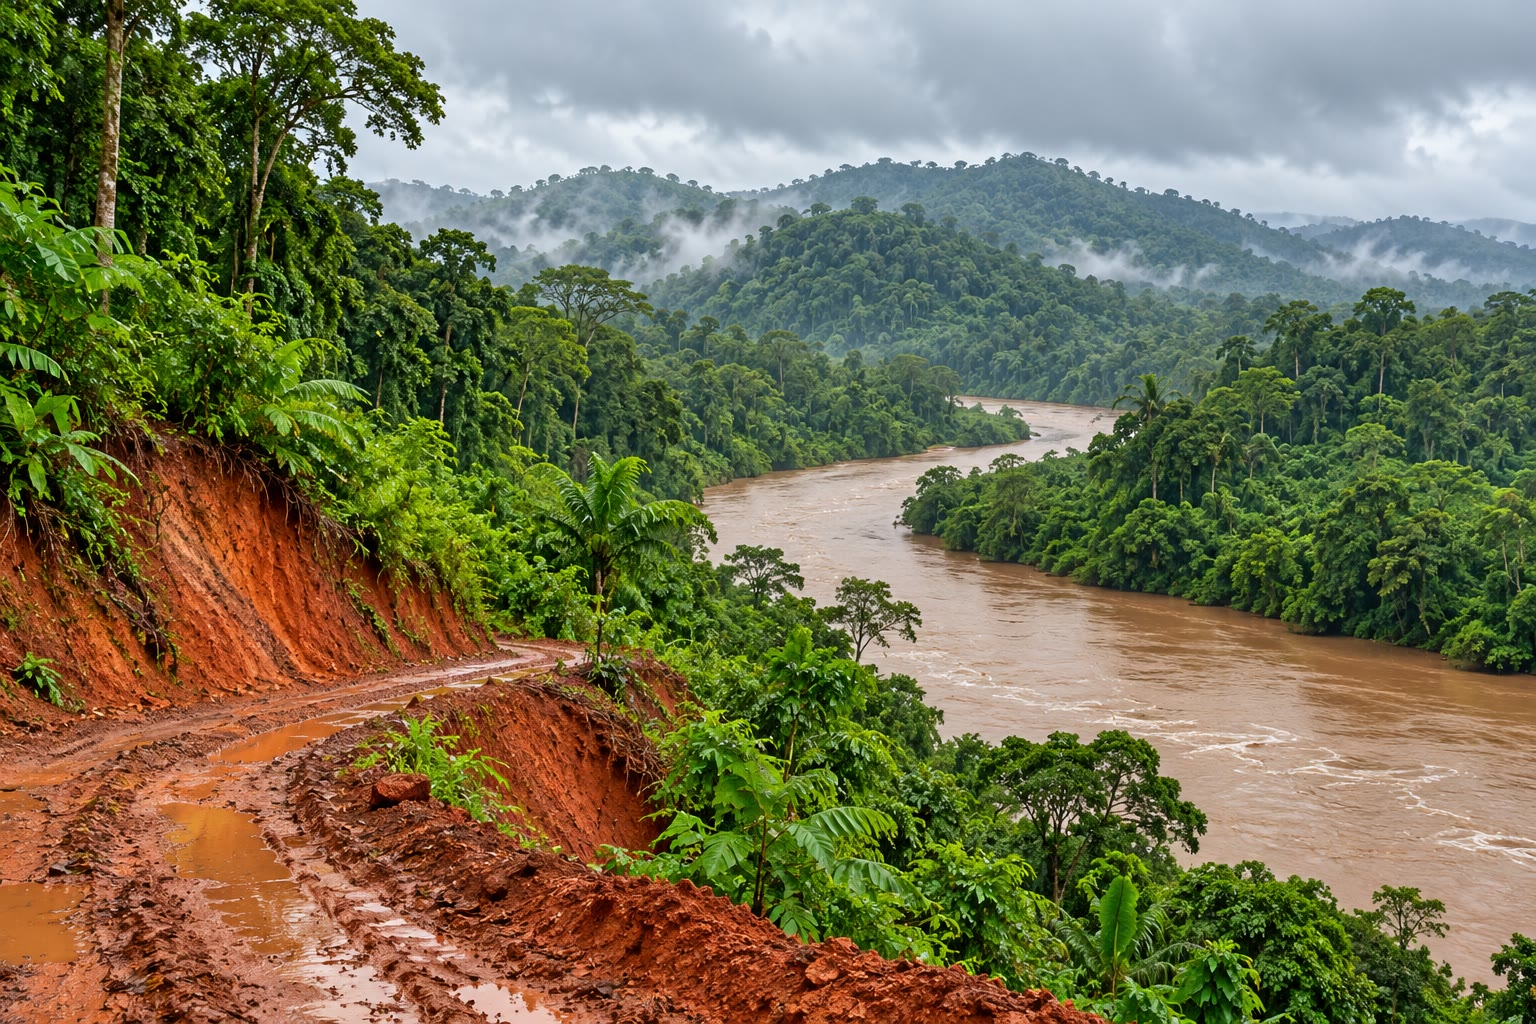
\includegraphics[width=0.66\linewidth]{images/book4/ai/b2-tropical-weathering.jpg}
\par\smallskip{\small Onde o termostato trabalha mais: uma planície quente e úmida, onde a chuva cai sobre
um solo vermelho profundamente intemperizado e o rio leva os produtos do intemperismo para o mar
(ilustração gerada por IA).}
\end{omfigure}

\section*{Exercícios}\label{sec:b2:deep-time-climate:exercises}

Dados para os exercícios, salvo indicação em contrário: carbono pré-industrial na atmosfera
\qty{591}{PgC} (\qty{278}{ppm}); $\qty{1}{Tmol}$ de carbono $= \qty{0.012011}{PgC}$; intemperismo dos
silicatos $W_0 = \qty{0.138}{PgC.yr^{-1}}$; fração de um excesso que fica no ar depois do oceano e dos
carbonatos $f = 0.08$; sensibilidade do intemperismo $k_T = \qty{0.09}{K^{-1}}$; sensibilidade climática $S =
\qty{3}{K}$; forçamento de uma duplicação do dióxido de carbono \qty{3.93}{W.m^{-2}}; $R =
\qty{8.314}{J.mol^{-1}.K^{-1}}$.
% ledger: ar6ch5:fig512, ipcc:erf-2xco2, derry24:fluxes, colbourn13:timescale, colbourn13:weathering, ipcc:ecs

\begin{exercise}[$\star$]\label{exo:b2:deep-time-climate:1}
Antes da era industrial o oceano continha \qty{900}{PgC} em sua camada superficial, \num{37100} em suas
águas intermediárias e profundas, 700 como carbono orgânico dissolvido e 3 em seus organismos vivos.
(a) Quanto carbono continha o oceano, e quantas vezes o da atmosfera? (b) Converta os
\qty{3.5e6}{Tmol} dos reservatórios superficiais em petagramas de carbono. (c) Que fração dele está no
ar?
\end{exercise}

\begin{exercise}[$\star$]\label{exo:b2:deep-time-climate:2}
Use os fluxos da figura do \omterm{def:b2:deep-time-climate:carbon-cycle}{ciclo do carbono de longo prazo}, com a desgaseificação metamórfica tomada como
\qty{3}{Tmol.yr^{-1}}. (a) Some as entradas nos reservatórios superficiais e as saídas.
(b) Que fração das entradas fornecem os vulcões, os riftes e o \omterm{def:b2:metamorphic-facies:metamorphism}{metamorfismo}? (c) Encontre o tempo de residência
do carbono nos reservatórios superficiais, usando as saídas.
\end{exercise}

\begin{exercise}[$\star$]\label{exo:b2:deep-time-climate:3}
(a) Escreva o intemperismo da forsterita, \ce{Mg2SiO4}, pelo dióxido de carbono e pela água em íons magnésio
e bicarbonato e sílica dissolvida, \ce{SiO2}, e balanceie-o. (b) O magnésio é depositado mais tarde
como carbonato. Escreva a reação líquida. (c) Que massa de forsterita precisa sofrer intemperismo para
remover \qty{1}{PgC} definitivamente? ($M(\ce{Mg2SiO4}) = \qty{140.7}{g.mol^{-1}}$.)
\end{exercise}

\begin{exercise}[$\star$]\label{exo:b2:deep-time-climate:4}
Ponha em ordem de idade, com suas datas, e diga para cada um se a Terra estava num estado de estufa ou de
refrigerador: o Ótimo Climático do Eoceno Inicial; a glaciação hirnantiana; o início do manto de gelo
antártico; o Turoniano; a maior extensão do gelo neopaleozoico; os grandes
avanços dos mantos de gelo do norte; o PETM.
\end{exercise}

\begin{exercise}[$\star\star$]\label{exo:b2:deep-time-climate:5}
(a) Verifique que uma energia de ativação de \qty{63}{kJ.mol^{-1}} a \qty{288}{K} dá $k_T =
\qty{0.09}{K^{-1}}$. (b) Encontre $k_T$ para o valor de campo \qty{74}{kJ.mol^{-1}}. (c) Com cada um, encontre
o aquecimento estacionário quando a desgaseificação aumenta \qty{20}{\percent}. (d) Por que a sensibilidade
climática não entra em (c)?
\end{exercise}

\begin{exercise}[$\star\star$]\label{exo:b2:deep-time-climate:6}
Compare o fator de Arrhenius exato $\exp[-(E_{\text a}/R)(1/T - 1/T_0)]$ com $e^{k_T(T -
T_0)}$, $k_T = E_{\text a}/(RT_0^2)$, para $E_{\text a} = \qty{63}{kJ.mol^{-1}}$ e $T_0 =
\qty{288}{K}$: (a) a $T = \qty{293}{K}$; (b) a $T = \qty{318}{K}$. (c) Mostre que a razão entre a
aproximação e o fator exato é $\exp[E_{\text a}x^2/(RT_0^2(T_0 + x))]$, com $x = T - T_0$,
e encontre o aquecimento para o qual ela atinge 1.1.
\end{exercise}

\begin{exercise}[$\star\star$]\label{exo:b2:deep-time-climate:7}
A compilação suavizada dá \qty{1444}{ppm} de dióxido de carbono a \qty{419.5}{Ma} e
\qty{276}{ppm} no fim de seu registro. (a) Encontre o forçamento desse declínio. (b) Compare-o com
os \qty{9}{W.m^{-2}} do Sol que se torna mais brilhante. (c) Encontre a taxa média de declínio em ppm por milhão de
anos, e compare-a com os \qty{3.4}{ppm} da tendência ajustada. Por que podem diferir?
\end{exercise}
% ledger: data:b4-foster2017, foster17:co2

\begin{exercise}[$\star\star$]\label{exo:b2:deep-time-climate:8}
(a) Distribua \num{3000} e \qty{7000}{PgC} ao longo de 3 e de \qty{20}{kyr}: que faixa de taxas de
liberação resulta? Compare com os 0.3 a \qty{1.5}{PgC.yr^{-1}} que o IPCC cita. (b) As emissões humanas
foram de cerca de \qty{35}{Gt} de dióxido de carbono em 2010. Converta em carbono e compare. (c) O dióxido de
carbono subiu de 900 para \qty{2000}{ppm}. Encontre o forçamento e o aquecimento de equilíbrio com $S =
\qty{3}{K}$, e compare com os \qty{5}{\celsius} de aquecimento sobre o clima anterior ao PETM.
\end{exercise}
% ledger: ar6ch5:petm-release, usgs:volcanic-co2, ar6ch5:petm

\begin{exercise}[$\star\star$]\label{exo:b2:deep-time-climate:9}
O soerguimento de uma cadeia de montanhas multiplica a intemperabilidade $W_0$ da Terra por 1.2, com
desgaseificação constante. (a) Encontre a nova variação estacionária de temperatura. (b) Encontre o novo
dióxido de carbono estacionário, a partir de \qty{278}{ppm}. (c) A taxa de intemperismo dos silicatos, no novo
estado estacionário, difere da antiga? Explique.
\end{exercise}

\begin{exercise}[$\star\star\star$]\label{exo:b2:deep-time-climate:10}
(a) Encontre o tempo de decaimento do termostato com o fator de escoamento, $k = 0.09 + 0.65\times0.045$.
(b) Ao longo de milhões de anos os mantos de gelo e a vegetação também respondem; com uma sensibilidade do sistema
terrestre de \qty{8}{K} por duplicação em vez de $S$, encontre $\tau$ com $k_T$. (c) Em que sentido as
duas mudanças empurram o termostato, e qual incerteza, $E_{\text a}$ ou $S$, importa mais?
\end{exercise}

\begin{exercise}[$\star\star\star$]\label{exo:b2:deep-time-climate:11}
Uma liberação de \qty{5000}{PgC} (depois do oceano e dos carbonatos). (a) Encontre o dióxido de carbono do
ar, em ppm, e o aquecimento. (b) Encontre a taxa líquida inicial de remoção $W - W_0$, e o tempo que o
pulso levaria para desaparecer a essa taxa. (c) Encontre o tempo linearizado para remover \qty{90}{\percent}
do excesso. (d) O modelo, integrado sem linearizar, leva \qty{340}{kyr}. Por que mais tempo?
\end{exercise}

\begin{exercise}[$\star\star\star$]\label{exo:b2:deep-time-climate:12}
(a) Linearize o modelo em torno de um estado estacionário em que a desgaseificação é $V$ e $C = C^*$, e mostre que
o tempo de decaimento é $\tau' = A_0 (C^*/C_0)\ln 2/(f k S V)$. (b) Calcule-o para o estado estacionário
de um aumento de \qty{20}{\percent} na desgaseificação. (c) O termostato é mais rápido ou mais lento num mundo rico em
dióxido de carbono, e por quê?
\end{exercise}

\begin{problem}[{Problema de fim de semana --- quanto tempo leva o termostato?}]\label{pb:b2:deep-time-climate:1}
Este problema constrói a constante de tempo do termostato a partir de fluxos medidos. Use os dados dos
exercícios; desgaseificação nas dorsais, \omterm{def:b2:oceanic-islands:stages}{ilhas oceânicas}, arcos e riftes \num{1.3}, \num{1.3}, 4.5 e
\qty{4.2}{Tmol.yr^{-1}}; intemperismo dos silicatos 11 a \qty{12}{Tmol.yr^{-1}}; energia de ativação
\qty{63}{kJ.mol^{-1}} a $T_0 = \qty{288}{K}$; massa da atmosfera \qty{5.1e18}{kg}, massa molar média
do ar \qty{28.97}{g.mol^{-1}}. Arredonde a três algarismos significativos.

\noindent\textbf{Parte I --- Balanço.}
\begin{enumerate}
  \item Some a desgaseificação vulcânica e dos riftes, em \unit{Tmol.yr^{-1}} e em \unit{PgC.yr^{-1}}.
  \item Tome $W_0$ no meio de sua faixa; converta-o em \unit{PgC.yr^{-1}}.
  \item Compare os dois. O que a comparação sugere sobre o \omterm{def:b2:deep-time-climate:carbon-cycle}{ciclo do carbono de longo prazo}?
  \item Quantos mols de ar contém a atmosfera? Quantos mols de carbono são \qty{591}{PgC},
        e que razão de mistura é essa?
  \item Sem nenhum intemperismo, quanto tempo levaria a desgaseificação da questão 1 para acrescentar
        \qty{591}{PgC} aos reservatórios superficiais?
  \item Se uma fração $f = 0.08$ disso ficasse no ar, por que fator subiria o dióxido de carbono
        do ar?
\end{enumerate}

\noindent\textbf{Parte II --- Linearização.}
\begin{enumerate}[resume]
  \item Encontre $k_T$ a partir da energia de ativação, e verifique que ele arredonda para o
        \qty{0.09}{K^{-1}} usado abaixo.
  \item Por que fator cresce o intemperismo para um aquecimento de \qty{1}{K}?
  \item Escreva o aquecimento $\Delta T$ para um excesso $M$, e sua derivada em $M = 0$, em
        \unit{K.PgC^{-1}}.
  \item Encontre a derivada de $W$ em relação a $M$ em $M = 0$, em \unit{yr^{-1}}.
  \item Mostre que seu inverso é a constante de tempo $\tau$ da
        \cref{prop:b2:deep-time-climate:thermostat}.
  \item Quais dentre $f$, $k$, $S$ e $W_0$ tornam o termostato mais rápido quando aumentam?
\end{enumerate}

\noindent\textbf{Parte III --- A constante de tempo.}
\begin{enumerate}[resume]
  \item Calcule $\tau$.
  \item Calcule-a com o fator de escoamento, $k = \qty{0.119}{K^{-1}}$.
  \item Calcule-a com $k_T$ e uma energia de ativação de \qty{74}{kJ.mol^{-1}}.
  \item Compare esses valores com os \qty{200}{kyr} a \qty{1}{Myr} dos modelos com oceano explícito.
  \item Quantos tempos de decaimento cabem nos \qty{50}{Myr} do declínio cenozoico do dióxido de
        carbono? O que isso diz sobre o estado do ciclo do carbono durante o declínio?
  \item A \qty{16}{ppm} por milhão de anos, quanto muda o dióxido de carbono em um $\tau$?
\end{enumerate}

\noindent\textbf{Parte IV --- Uma liberação do tamanho do PETM.}
\begin{enumerate}[resume]
  \item São liberados \qty{5000}{PgC}; quanto fica no ar depois que o oceano e os carbonatos
        agiram, e qual é o dióxido de carbono em ppm?
  \item Encontre o aquecimento nesse momento.
  \item De quanto sobe a taxa de intemperismo, em \unit{PgC.yr^{-1}} e em porcentagem?
  \item Com a lei linearizada, quanto tempo até que \qty{90}{\percent} do excesso tenha desaparecido?
  \item O carbonato do PETM recuperou-se em cerca de \qty{100}{kyr}. Dê duas razões pelas quais a Terra
        real pode ter sido mais rápida que este modelo.
  \item Em resumo: qual é o tempo de decaimento do \omterm{def:b2:deep-time-climate:thermostat}{termostato do intemperismo dos silicatos} neste modelo?
\end{enumerate}
\end{problem}
% ledger: derry24:fluxes, colbourn13:weathering, colbourn13:timescale, ar6ch5:fig512, ar6ch5:petm, ar6ch5:cenozoic-co2, ipcc:ecs, earth:Matm, earth:Mmol
